In this chapter, a proposed extension to the broader "Automation and Intelligent Optimisation in High Performance Sailing Boats" project will be described. This Sail Trim Approach was my proposed master's thesis topic, but together with my supervisors, we decided to continue the Reinforcement Learning Approach instead.

\section{Introduction}
Sail trim is the biggest factor in the speed of the boat. An autopilot with a good sail trim would go faster than an expert human skipper with a bad sail trim. With a camera at the back of the boat looking at the main sail, we can train a model that can predict whether the main sail trim is good, too loose, or too tight.

Judging the sail trim is easy to a trained eye, but depending on the wind conditions, might require a lot of attention if the wind is gusty, or there is land or any obstacles nearby that might disturb the wind flow.
 
Full crews have dedicated people for sail trim, however it is hard to achieve constant good trim with shorthanded sailing with one or two people. This project would help shorthanded sailors, for cruising or racing, plus it can also be used for teaching sail trim to beginners.


\section{Literature Review}
In this section, a current overview of the relevant topics related to the proposed Sail Trim Approach (\ref{LR:TL}, \ref{LR:IG}, and \ref{LR:AST}) are presented. Transfer Learning is a suggested technique to be used in Sail Trim Approach so that the model can be trained with less collected data. Integrated Gradients is an Explainable AI technique which can be used for understanding what the sail trim model is learning to check if its correct. Lastly, Assisted Sail Trim is a system used in cruising yachts that is somewhat similar to the proposed Sail Trim Approach.

\subsection{Transfer Learning} \label{LR:TL}
Transfer learning is a method where a machine learning model trained for a task is used as a starting point for another task.\cite{brownlee_2019} In our context, instead of training a model from ground up, transfer learning can be utilized by building up on a model that was previously trained for a large scale image classification task. The idea behind transfer learning for imaging is that if a model is trained on a large and general enough dataset, it can serve as a generic model of the visual world. \cite{TF:TL} This generic model can be trained much more easily to classify different sail trims thanks to its advantages. 

Lisa Torrey and Jude Shavlik explain in their book the 3 advantages of transfer learning and how it improves model learning \cite{10.5555/1803899}, which can be seen in Figure \ref{fig:TL}.

\begin{figure}[h]
\centering
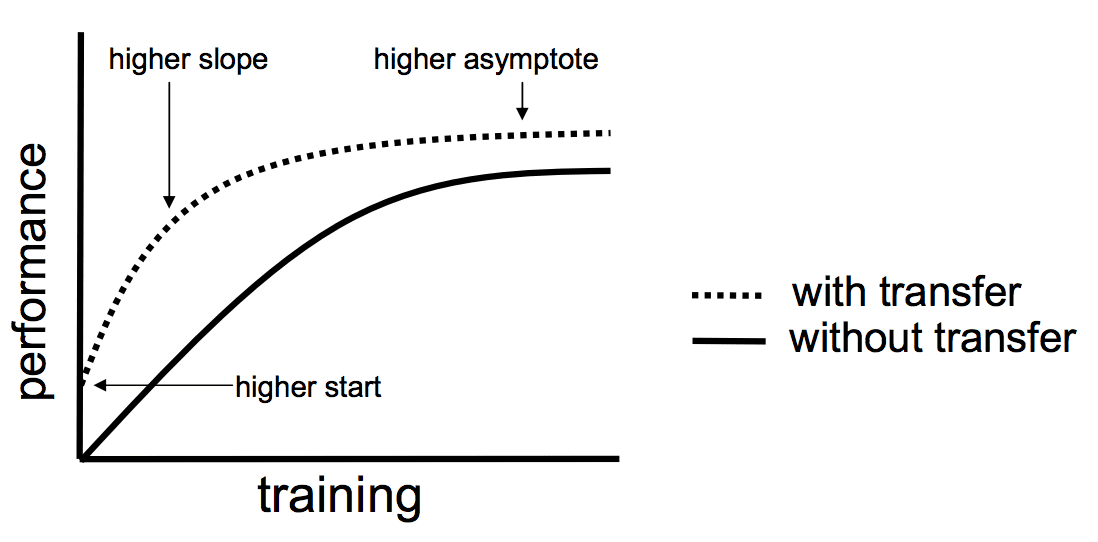
\includegraphics[width = 0.7\hsize]{figures/transfer-learning.png}
\caption{Transfer learning performance improvements \cite{10.5555/1803899}}
\label{fig:TL}
\end{figure}

\begin{enumerate}
  \item \textbf{Higher start:} The initial performance is better 
  \item \textbf{Higher slope:} The model improves faster 
  \item \textbf{Higher asymptote:} The converged performance is better 
\end{enumerate}

\begin{figure}[h]
\centering
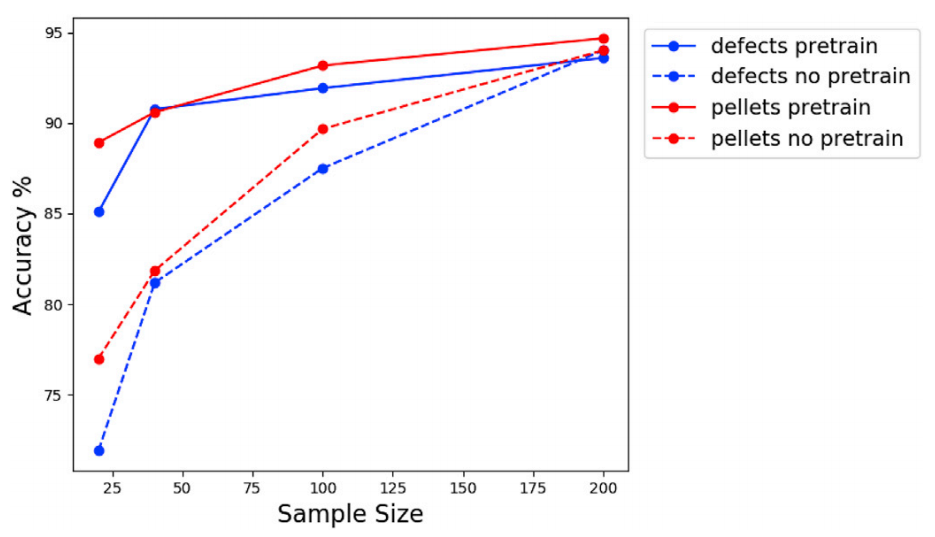
\includegraphics[width = 0.7\hsize]{figures/transfer learning results.png}
\caption{Affect of transfer learning on accuracy vs sample size \cite{ZHU2021104269}}
\label{fig:TL-results}
\end{figure}

Theoretically, using transfer learning the deep learning models converge much faster, as seen in Figure \ref{fig:TL}. This means that models can be trained with a lot less data. In their study, Wenbo et al. examines the transfer learning for image classification's impact on training sample size. \cite{ZHU2021104269} Wenbo et al. conclude that the deep learning models can achieve over 90\% accuracy for image classification tasks by using less than 100 samples utilizing transfer learning, significantly lower than the previous rule of thumb of 1000 samples per class. Wenbo et al.'s results graph of accuracy vs sample size, with and without transfer learning can be seen in Figure \ref{fig:TL-results}.

\subsection{Integrated Gradients} \label{LR:IG}
Integrated Gradients is an explainable AI technique to help understand what the model is learning, which can be used in any differentiable model such as images, text or structured data. \cite{TF:IG} The suggested usage in the sail trim approach is on images, to see whether the model is learning the expected features. The technique is easy to implement, and requires no modifications on the original network, only requires some calls to the standard gradient operator. \cite{IGpaper} An example of Integrated gradients used on images can be seen in Figure \ref{fig:IG}. 

\begin{figure}[h]
\centering
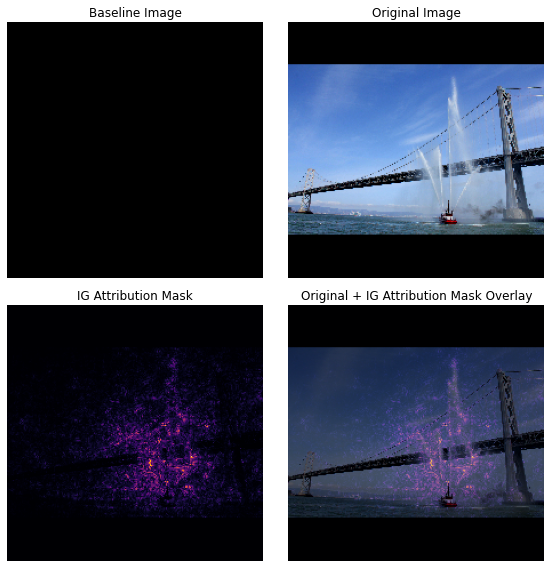
\includegraphics[width = 0.7\hsize]{figures/IG_fireboat.png}
\caption{Integrated Gradients example \cite{TF:IG}}
\label{fig:IG}
\end{figure}

When the models do not perform as expected, or just to see what the models have learned, Integrated Gradients is a nice technique to have to be able to understand and debug the models: either by regularization or gathering more and better balanced data.

\subsection{Jeanneau \& Harken Assisted Sail Trim} \label{LR:AST}
A somewhat similar idea to the sail trim approach has been done as a collaboration with Jeanneau and Harken in 2015, \cite{harkenAST} which won the Pittman Innovation Award. \cite{pittman_awards}
The Assisted Sail Trim (AST) system has several components. The relevant component to this project focuses on maintaining the rough trim of the sails by adjusting the sheets depending on the apparent wind measured by on-board electronics. An illustration of this can be seen in Figure~\ref{fig:AST}.

\begin{figure}[h]
\centering
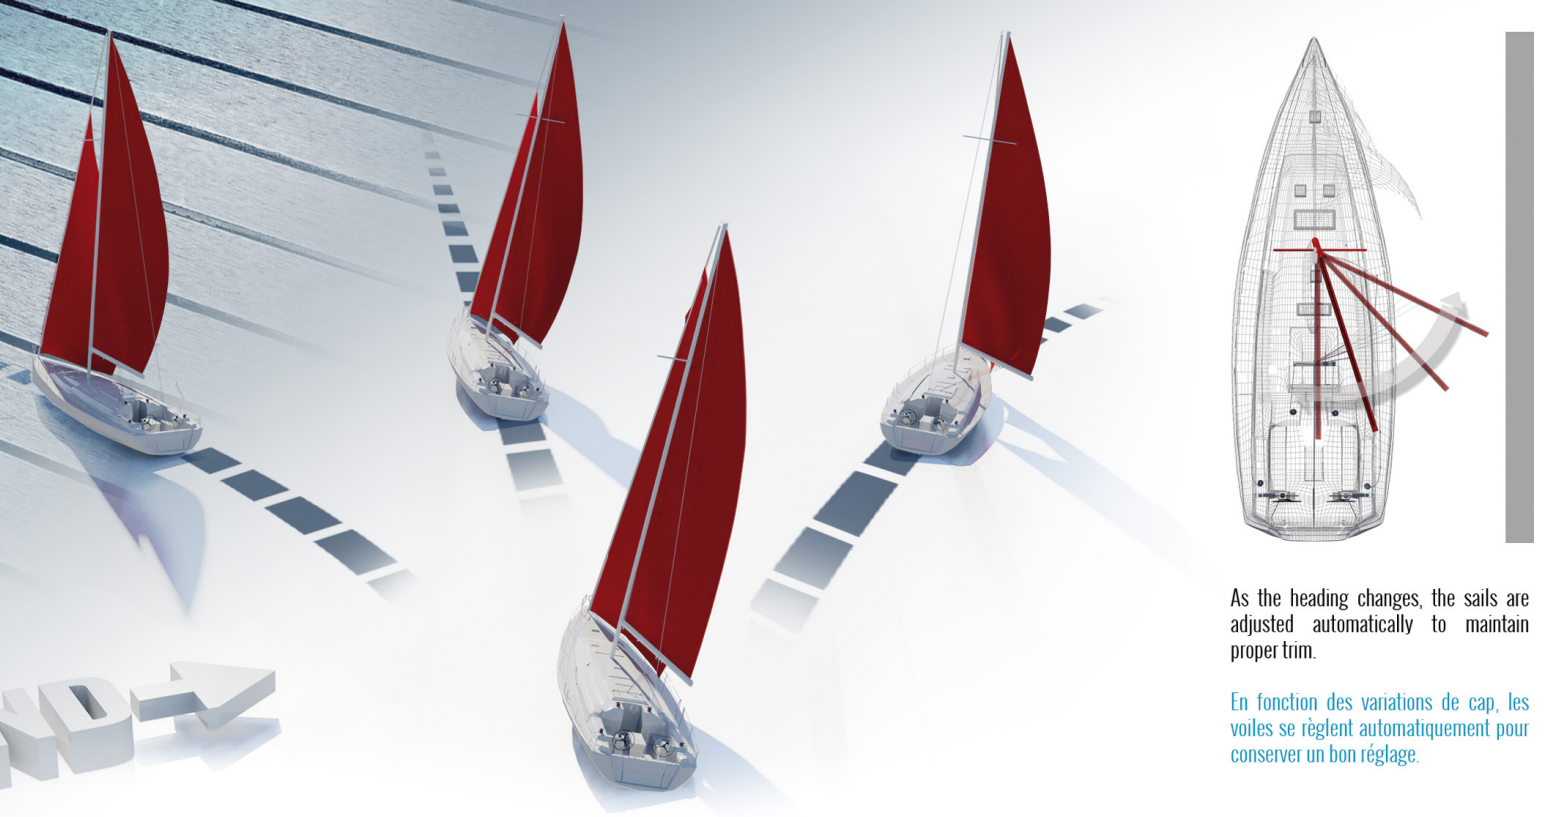
\includegraphics[width = \hsize]{figures/AST.png}
\caption{Assisted Sail Trim - apparent wind sail adjustment \cite{ASTbrochure}}
\label{fig:AST}
\end{figure}

AST is only available on the 2015 Jeanneau Sun Odyssey 519, and it is discontinued. It also did not utilize machine learning, required much more electronics and budget than a single camera, and it was specific to the sailboat, not transferable. In addition, the sails can have vastly different shapes even in similar sheet positions, resulting in great performance difference. The proposed sail trim approach focuses on the fine sail trim, rather than the coarse trim achieved in AST.

Another difference between AST and the suggested sail trim approach is that AST system can communicate with the winches, and automatically adjust the main sheet. Suggested sail trim approach will not communicate with the rest of the onboard electronics, and rely on the crew to take actions. Although this is less user friendly, it has its own advantages. Two use cases of the sail trim approach are education and competition. Making the crew do the trim by giving trim suggestion will be more educational than doing it for them. Plus automated sail trim is not allowed in some class rules, so this project can be used in competitions among wider sailboat classes.

\section{Sail Trim Background}
As explained in section \ref{LR:AST}, the sails can have vastly different shapes in similar boom and sheet positions as can be seen in Figure~\ref{fig:mainsail-trim}. There are a lot of reasons why a sail trim might be off. For example the sail might not be cut properly, or the mast position and mast bend might not be optimal for the weather conditions. But these are pretty unlikely, and most likely, it is the mainsail controls that can be adjusted on the go that cause bad trim. Below are some notable reasons of bad mainsail trim on the go.

\begin{figure}[h]
\centering
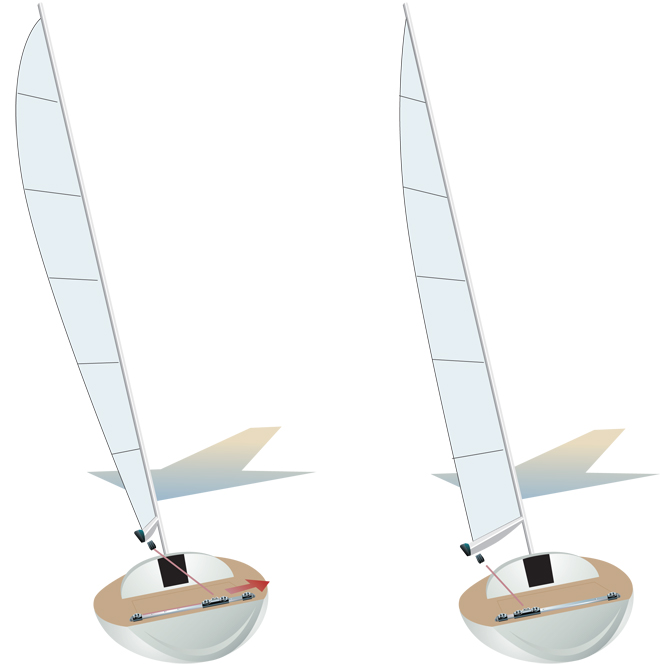
\includegraphics[width = 0.6\hsize]{figures/sail-trim-approach/mainsail-trim-back.jpg}
\caption{Good(left) and bad(right) light wind mainsail trim \cite{img:mainsail-trim-back}}
\label{fig:mainsail-trim}
\end{figure}

\noindent Main sail might be too strained because of:
\begin{itemize}
  \item The main sheet is pulled in too much
  \item Boom vang is too tight
  \item Main sail traveller is not utilized correctly
\end{itemize}

\noindent Main sail might be too loose because of:
\begin{itemize}
  \item The main sheet is not pulled enough
  \item Boom vang is too loose
  \item Main sail is not fully up to the top of the mast
\end{itemize}

There are other mainsail controls that affect the trim such as cunningham and outhaul, but those depend a lot on the boat class, and even in same boat class, different sailmakers have different suggestions on how to utilize them. The mentioned mainsail controls can be seen in Figure \ref{fig:mainsail-controls}.

\begin{figure}[h]
\centering
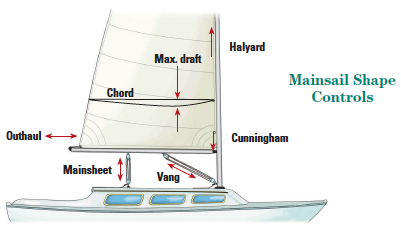
\includegraphics[width = 0.7\hsize]{figures/sail-trim-approach/mainsail-shape-controls.png}
\caption{Mainsail controls that affect trim \cite{img:mainsail-shape-controls}}
\label{fig:mainsail-controls}
\end{figure}

\section{Sail Trim Capture System}

The suggested camera placement is at the center back of the boat, possibly at the bimini top, as shows in Figure \ref{fig:camera-pos}. A camera from this angle will see a similar view of the sails with Figure \ref{fig:telltales}.

\begin{figure}[h]
\centering
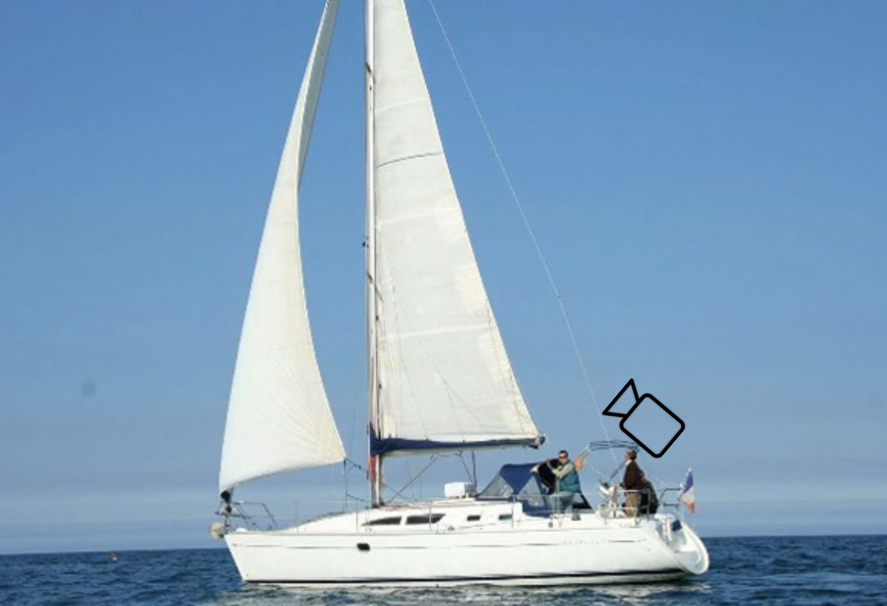
\includegraphics[width = 0.7\hsize]{figures/sail-trim-approach/camera-position.png}
\caption{Camera position}
\label{fig:camera-pos}
\end{figure}

\begin{figure}[h]
\centering
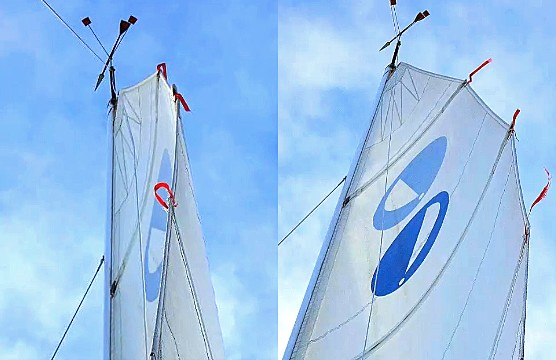
\includegraphics[width = 0.8\hsize]{figures/sail-trim-approach/telltales.jpg}
\caption{Camera's view of a bad(left) and good(right) light wind mainsail trim \cite{img:telltales}}
\label{fig:telltales}
\end{figure}

The easiest way to tell if the trim is good for a human is to look at the red telltales at the back of the sails, see Figure \ref{fig:telltales}. The most important one is the topmost one. If the telltales are flying straight back, it means that the air is coming out of the sails alright. However if the telltale is going to the back of the sails, it shows us that the wind flow at the back of the sails are not optimal, meaning the trim is sub-optimal and the sails need to be loosened.

For a machine, the easiest way to check trim might be comparing the areas of sail and the sky. In Figure \ref{fig:telltales}, you'll notice that Assuming a clear sky, by only comparing the number of blue pixels(sky) and the number of whiter pixels(sails), a very simple model can tell the difference between a good and a bad trim.

Using the state of the art image classification models, we can achieve much better results, theoretically learning the sail trim for different wind and weather conditions, apparent wind angles, maybe even across different boats.


\section{Suggested Timeline}

The suggested timeline and some additional details for this project, planned considering the available time for Imperial MSc thesis projects can be seen in Figures \ref{fig:sta-plan1} and \ref{fig:sta-plan2}.

\begin{figure}[h]
\centering
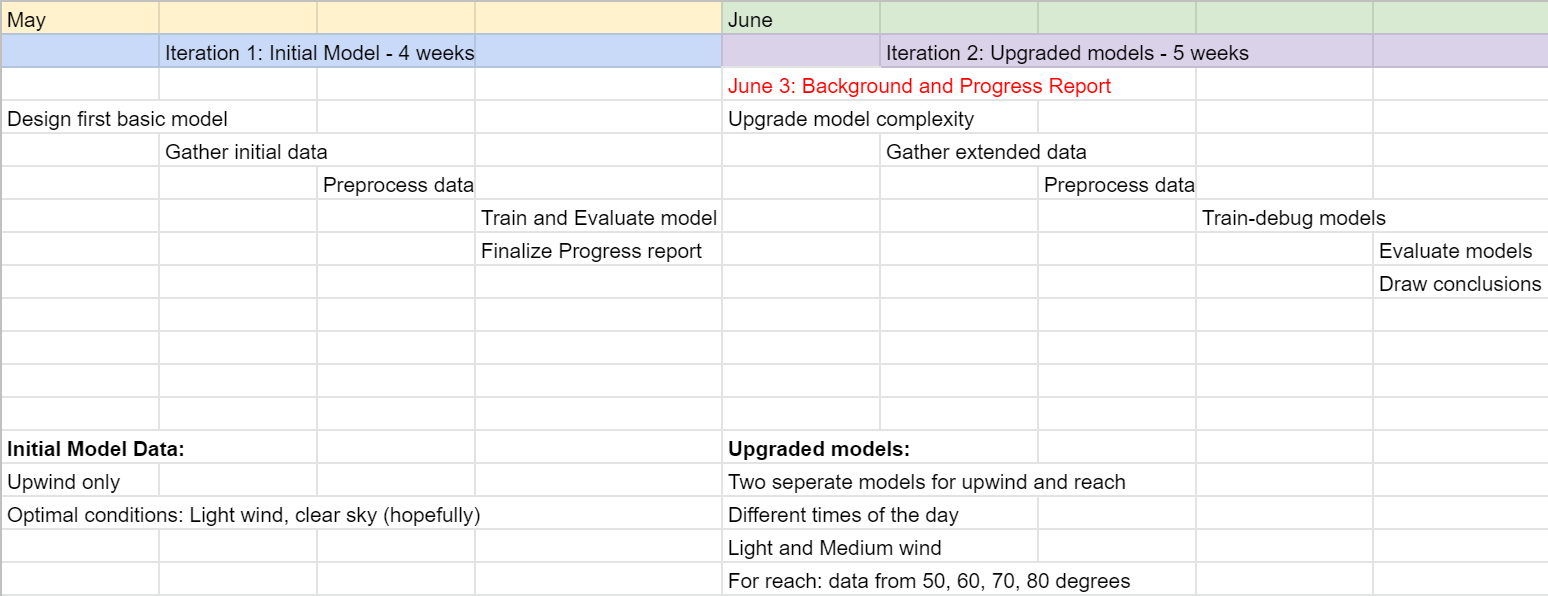
\includegraphics[width = \hsize]{figures/sail-trim-approach/plan1.png}
\caption{Suggested plan - Iterations 1 and 2}
\label{fig:sta-plan1}
\end{figure}

Iteration 1 aims to build a simple Proof of Concept that machine learning models can classify good and bad sail trims. After the initial Proof of Concept, the models are extended in Iteration 2. If the expected results are not met in the first iteration, using Integrated Gradients explained in section \ref{LR:IG}, one can see what the models have learned, assess if the learnt features are correct, and balance the dataset with more data countering the false features.

\begin{figure}[h]
\centering
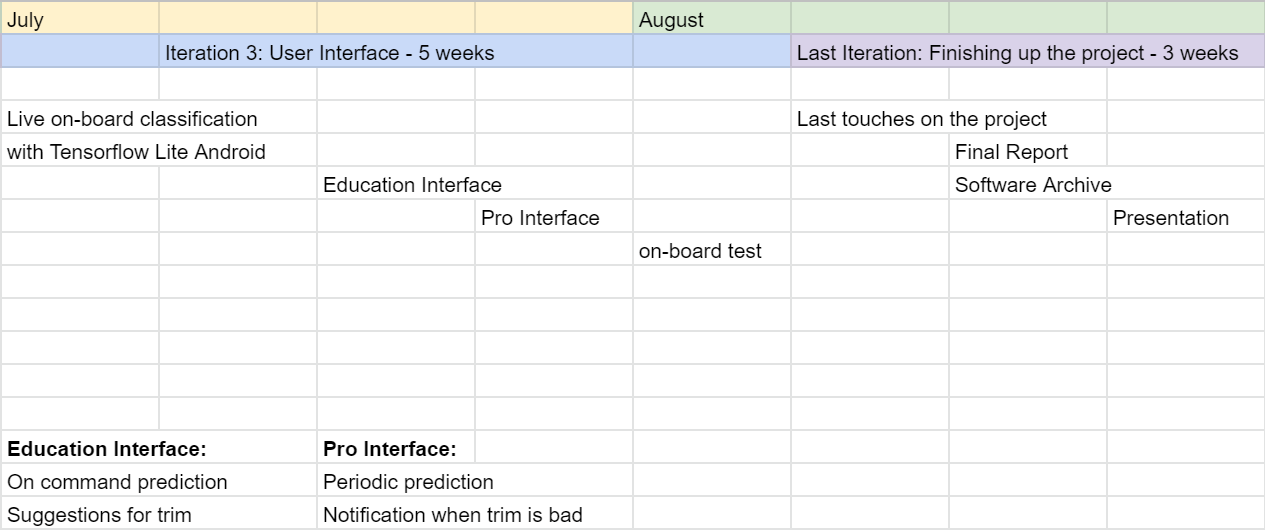
\includegraphics[width = \hsize]{figures/sail-trim-approach/plan2.png}
\caption{Suggested plan - Iterations 3 and 4}
\label{fig:sta-plan2}
\end{figure}

Iteration 3 aims to implement the models live on-board using a smartphone, including two different interfaces for education and professional use cases. Iteration 4 contains a buffer week if anything goes wrong for the project, then some time for project submission preparations, namely the code submission to software archive, final report, and the final presentation.

For more information about the Sail Trim Approach, you can email me at:\\
\href{mailto:doruktaneli97@gmail.com}{doruktaneli97@gmail.com}